\chapter{Segmentation}

当图片出现不同的对象(例如同时出现猫狗),那么能否将属于同类的pixel分到一起?Not a global label.

Image segmentation:将图片分割为连贯的各个对象,不关心其语义.经典方法:grouping and clustering.
后者就是指将相似的数据点分为一组,然后给予它们一个标识符.

clustering-based segmentation:对于实际图片,颜色当然不可能如此理想.
因此我们要选取三个"中心"来代表,然后将每个pixel以离其最近的中心作为标记.

目标函数:
\begin{equation}
	c^*, \delta^* = \arg \min_{c, \delta} \frac{1}{N} \sum_{j}^{N} \sum_{i}^{k} \delta_{ij} (c_i - x_j)^2.
\end{equation}

很难求解.

很多时候,这个问题是一个"先有鸡还是先有蛋"的问题.即何者优先?

破解之法:如果我们提前知道有$k$个center,则可以调用kmeans.实际就是random initialization.

coordinate decent是一个启发式策略(先找一个方向的最小值,然后下降).但无论如何,kmeans对于初始化非常敏感.它必须提前知道几个group,
并且是无监督的.kmeans实际上进行了对intensity进行了quantum.除此之外还有mean shift.\footnote{其实没人会拿intensity做kmeans.
因为intensity显然不能体现pixel的相关性.}

总结:grouping-based:只关心局部,不关心语义,不可能达到high-level.是bottom-up的方法.而神经网络则是top-down的.

由于纯粹的Instance segmentation已经极为少见,因此今天提及这个词,多是带语义的.

我们今天的问题:Semantic segmentation.实际上就是对每个pixel进行classification.

segmentation时候的一大问题:对每个patch,分类极度依赖上下文.(纯黑的牛)因此,将每个pixel割裂开是不可能实现分类的.

原先的神经网络:图像->padding/strided cnn->拉成vector->MLP->softmax->类别信息.
这是一个不断提取特征的过程.但在segmentation当中,
我们的输出应该与输入一样大.怎么把feature map先变小再变大?
我们的想法是:先缩小提取特征(两头牛),然后回到原图上以此为原则,寻找.

\begin{wrapfigure}{r}{4cm}
	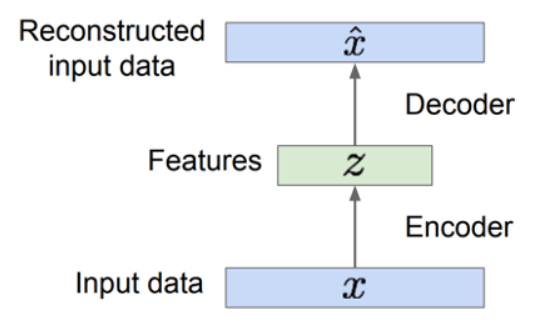
\includegraphics[scale=0.5]{figures/autoencoder.png}
	\caption{name of the figure}
\end{wrapfigure}
NN核心概念:Auto-Encoder.自监督.定义reconstruction loss
\begin{equation}
	\tnorm{\bm x - \hat{\bm{x}} }
\end{equation}

Encoder MLP $f:\mathbb R^m \to \mathbb R^h, h \ll m$.decoder:$g:\mathbb R^h \to \mathbb R^m$.
对于$H \times W \times 3$的图像,实际维度到不了这么多.因此可以进行encode.

考虑classification:$\mathbb R^{H \times W \times 3} \to \{0, 1\}^{k}$.
这样我们就用一个词表示了原图.同样,对于Auto-Encoder,
也是如此,即我不相信这么多像素都是独立分布,
应该是$H \times W \times 3$空间的低维曲面.
同样对于segmentation,我们希望从原图到特征map,然后回到原图,获得分类,而不需要原图的RGB信息.

In-Network Unsamping:Unpooling.

第一种是copy-paste,需要用conv对raw unsamping image进行处理.

In-Network Unsamping:Max Unpooling:记住哪个位置是池化中最大的.
也就是说,并不是所有信息都在bottle neck(中间小的部分)处.这也需要进行大量conv加工.

能不能在一步之内完成?Learnable unsampling:Transpose convolution.
学习出来一个conv,从$2 \times 2 \to 4 \times 4$.Fully Convolutional Network.
全都是Conv进行降采样和升采样.

每一次把feature map变小,后面层的conv的reception field都会变大,
比不做dimentional reduce的图片感受野更大.
有助于提取global context.bottleneck的双重意义:增大感受野,减小size.

关键:增大感受野,收缩image从而集中特征,去除无用.

\begin{wrapfigure}{r}{6cm}
	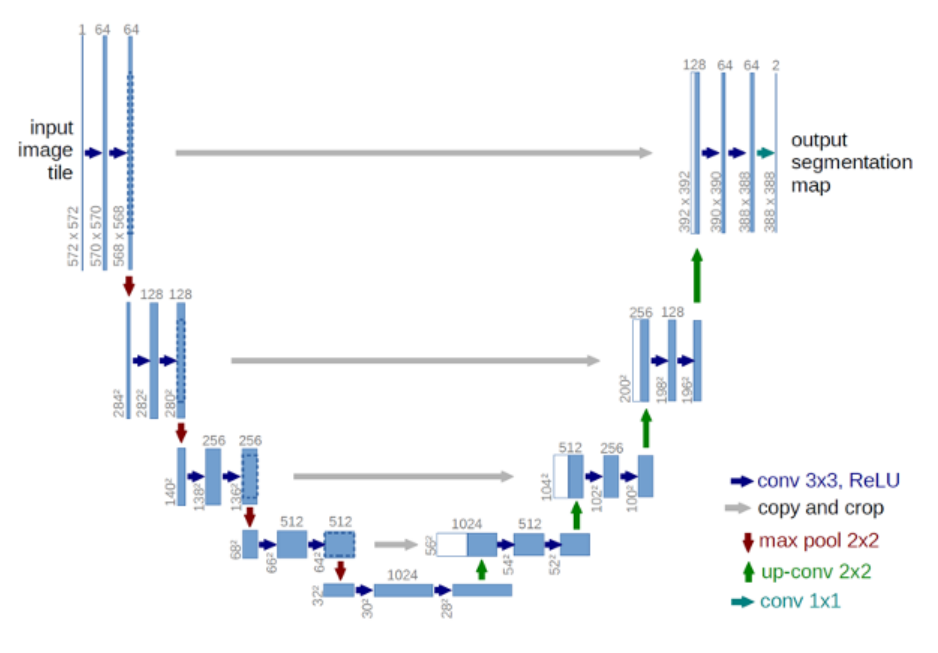
\includegraphics[scale=0.4]{figures/UNetstructure.png}
	\caption{UNet的结构示意图}
\end{wrapfigure}

那么FCN有什么问题呢?我们先来看看它的bottle neck存储了什么?降低resolution,多个channel.
现在在neck里面的内容本来就不多,你还要求通过相同的升采样之后,还能还原出boundary,
这件事与classification相比,不是一句话能说完的,neck里恐怕很难同时存储下特征和原图的boundary信息.


那么我们让各个层次的resolution经过几层conv\footnote{前几层可以理解为在寻找corner和edge.}
直接连接到对称的升维操作,照着把bound画出来就可以,中间neck就只需要记context了.
这是一个非常经典的结构,被称为UNet,也是如今Segmentation乃至depth detection,
dense prediction都需要参考的结构,甚至也是Diffusion model\footnote{但是非常有趣的是U-net最初是在生物学语义分割中提出的.2024笔者注}的一个重要的 Backbone.


Evaluation Metrics: Pixel Accuracy.

\begin{equation}
	\text{accuracy} = \frac{TP+TN}{TP+TN+FP+FN}
\end{equation}

当然这很有问题:比如一个人头只占据整个图片,那么将整个图片预测为背景,那么错误率也很低,但是这很显然不对.

另一个loss:IoU->mean of every class IoU -> soft IoU.